\section{Analityczny regulator predykcyjny MPCS}
Do obliczeń regulatora predykcyjnego MPCS wykorzystano model liniowy obiektu w oparciu o równania stanu postaci zgodnej z równaniem \ref{equation:defaultdss}. Wektor stanu $x$ i wejścia $u$ odpowiadał zmiennym zgodnie z równaniem \ref{equation:defineddss}. Po wykonaniu obliczeń, współczynniki macierzy $A$, $B$, $C$, oraz $D$ wynosiły tyle ile na równaniu \ref{equation:matricesdvals}. Zmienna $k_{const_0}$ odpowiada dodatkowej stałej dodawanej do obliczeń objętości, jest ona nieistotna dla pracy regulatora. Należy zauważyć, że zmienną wyjściową modelu jest zmienna $V$. Ponieważ znana jest zależność między $V$ a $H$, zamiana z jednej zmiennej na drugą jest prosta. Pojawia się za to problem uwarunkowania macierzy $B$. Wartości objętości są o około 2 rzędy większe niż wartości temperatury. Dlatego regulator wykonuje obliczenia na modelu o $100$ krotnie zmniejszonej objętości, a więc także o $100$ krotnie zmniejszonym pierwszym wersie macierzy $B$, regulator nie bierze również pod uwagę wejść niesterowalnych, macierz $B$ wykorzystywana przez regulator ma więc postać $B_{reg}$, zgodnie ze wzorem \ref{equation:bregval}. Ogólna struktura regulacji przedstawiona jest na Rys. \ref{fig:mpcs}. Na wykresach pokazane jest działanie regulatora dla przykładowego przebiegu wartości zadanych, różnych wartości horyzontów $N$ i $N_u$, oraz parametru $\lambda$, dla obiektu określonego liniowymi równaniami stanu oraz dla obiektu nieliniowego zdyskretyzowanego metodą rk4. Przyjęto wartości sterowania w zakresie $\langle 0 : 100 \rangle$, oraz maksymalną zmianę sterowania w jednej chwili $k$ za $\pm0.2$. Należy zauważyć, że zmienna $T$ obarczona jest znacznym błędem linearyzacji. Jak można zauważyć na podstawie wykresów, regulator MPCS charakteryzuje się niewielkim uchybem ustalonym dla zmiennej $T$, może on wynikać z błędu linearyzacji. Poza tym problemem, regulator działa bardzo dobrze nawet z ograniczeniami, dla horyzontów o wartościach na poziomie kilkuset próbek. Wartości zmiennych sterowanych szybko zbiegają do wartości zadanych, a przeregulowania są względnie niewielkie. Dla dużych zmian wartości zadanych jednak regulator ten nie może być dobrze zastosowany, ze względu na błędy wynikające z linearyzacji obiektu. Oczywiście obiekt oparty o równania przestrzeni stanu nie jest obarczony tymi problemami i regulacja w jego przypadku jest niemal idealna. Na ostatnim wykresie przedstawiono również działanie regulatora dla zmiennego zakłócenia $F_d$. Jak widać, nie radzi on sobie zbyt dobrze ze zmiennym zakłóceniem.


\begin{equation}
\label{equation:defaultdss}
\begin{aligned}
    x(k+1) = & Ax(k) + Bu(k) \\
    y(k) = & Cx(k) + Du(k)
\end{aligned}
\end{equation}

\begin{equation}
\label{equation:defineddss}
    \begin{aligned}
        x = &
        \begin{bmatrix}
            V \\
            T 
        \end{bmatrix}\\
        u = &
        \begin{bmatrix}
            F_H \\
            F_C \\
            F_D \\
            T_H \\
            T_C \\
            T_D
        \end{bmatrix}
    \end{aligned}
\end{equation}

\begin{equation}
\label{equation:matricesdvals}
    \begin{aligned}
        k_{const_0} &= -47.25\\
        A = &
        \begin{bmatrix}
            0.9966 & 0\\
            -4.23e-09 & 0.9864\\
        \end{bmatrix} \\
        B = &
        \begin{bmatrix}
            0.9983 & 0.9983 & 0.9983 & 0 & 0 & 0\\
            0.006148 & -0.002286 & -0.0001233 & 0.003028 & 0.008001 & 0.002595\\
        \end{bmatrix}\\
        C = &
        \begin{bmatrix}
            1 & 0\\
            0 & 1
        \end{bmatrix}\\
        D = & 
        \begin{bmatrix}
            0 & 0 & 0 & 0 & 0 & 0 \\
            0 & 0 & 0 & 0 & 0 & 0 
        \end{bmatrix}
    \end{aligned}
\end{equation}

\begin{equation}
\label{equation:bregval}
    \begin{aligned}
        B_{reg} = &
        \begin{bmatrix}
            0.009983 & 0.009983\\
            0.006148 & -0.002286\\
        \end{bmatrix}\\
    \end{aligned}
\end{equation}

\begin{figure}[h!]
   \centering
   \includegraphics[scale=0.7]{img/MPCSanaRK/MPCSDiag.pdf}
   \caption{Ogólny schemat regulacji z wykorzystaniem algorytmu MPCS}
   \label{fig:mpcs}
\end{figure}


\FloatBarrier
    \begin{figure}[h!]
   \centering
   \begin{subfigure}[b]{0.4\textwidth}
      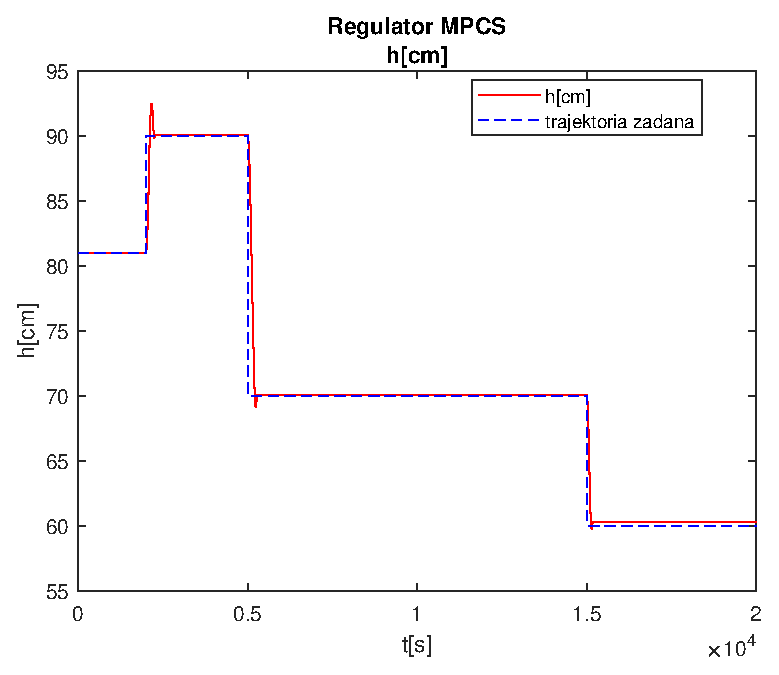
\includegraphics[width=1\linewidth]{img/MPCSanaRK/MPCSRKHN50Nu10l100.eps}
      \caption{}
      \label{fig:fig:MPCSRKN50Nu10l1001}
   \end{subfigure}
       
   \begin{subfigure}[b]{0.4\textwidth}
      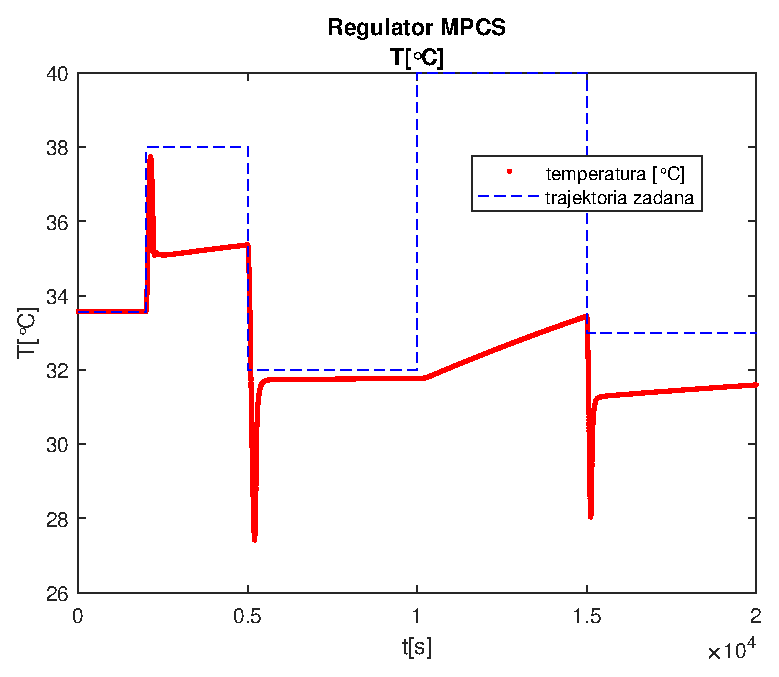
\includegraphics[width=1\linewidth]{img/MPCSanaRK/MPCSRKTN50Nu10l100.eps}
      \caption{}
      \label{fig:fig:MPCSRKN50Nu10l1002}
   \end{subfigure}
       
   \begin{subfigure}[b]{0.4\textwidth}
      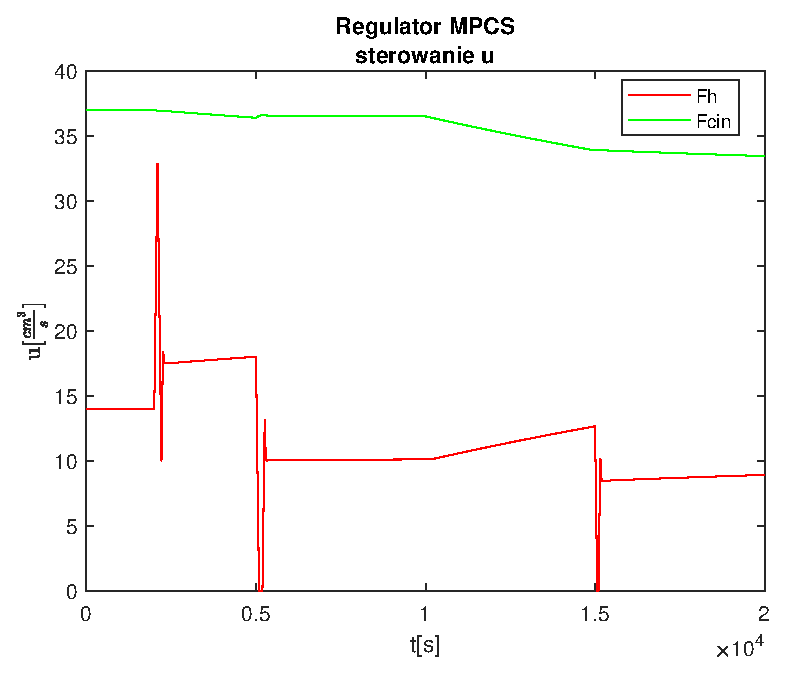
\includegraphics[width=1\linewidth]{img/MPCSanaRK/MPCSRKControlN50Nu10l100.eps}
      \caption{}
      \label{fig:fig:MPCSRKN50Nu10l1003}
   \end{subfigure}
       
   \caption{Wykresy dla regulatora MPCS, obiekt nieliniowy, $N = 50$, $N_u = 10$, $\lambda = 1$ .}
   \label{fig:MPCSRKN50Nu10l100}
\end{figure}
           

\FloatBarrier

\FloatBarrier
    \begin{figure}[h!]
   \centering
   \begin{subfigure}[b]{0.4\textwidth}
      \includegraphics[width=1\linewidth]{img/MPCSanaLin/MPCSLinHN300Nu100l10.eps}
      \caption{}
      \label{fig:fig:MPCSLinN300Nu100l101}
   \end{subfigure}
       
   \begin{subfigure}[b]{0.4\textwidth}
      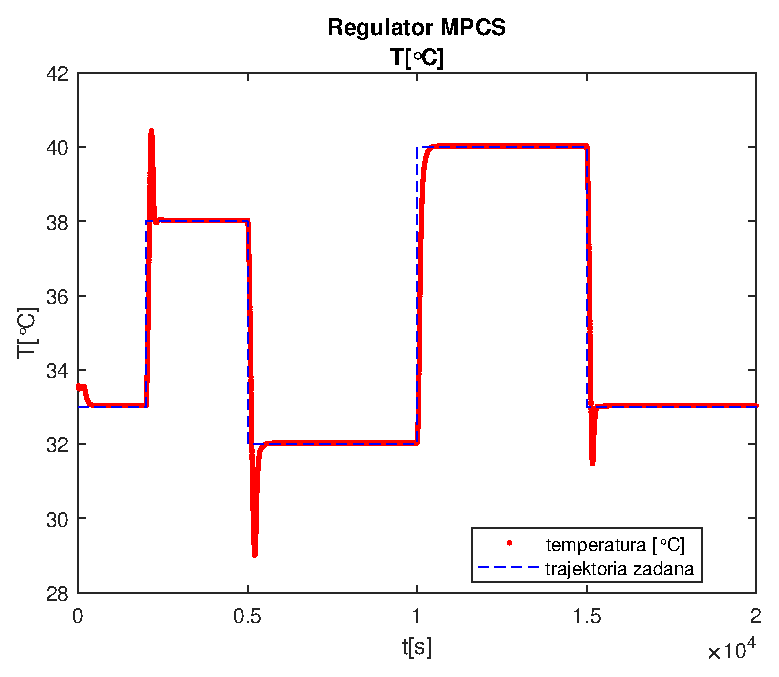
\includegraphics[width=1\linewidth]{img/MPCSanaLin/MPCSLinTN300Nu100l10.eps}
      \caption{}
      \label{fig:fig:MPCSLinN300Nu100l102}
   \end{subfigure}
       
   \begin{subfigure}[b]{0.4\textwidth}
      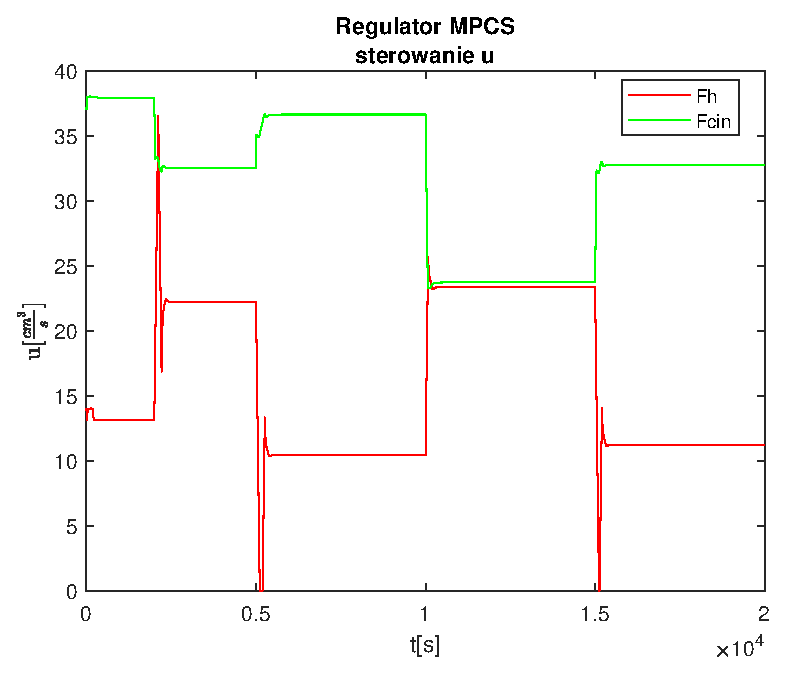
\includegraphics[width=1\linewidth]{img/MPCSanaLin/MPCSLinControlN300Nu100l10.eps}
      \caption{}
      \label{fig:fig:MPCSLinN300Nu100l103}
   \end{subfigure}
       
   \caption{Wykresy dla regulatora MPCS, obiekt liniowy, $N = 300$, $N_u = 100$, $\lambda = 0.1$.}
   \label{fig:MPCSLinN300Nu100l10}
\end{figure}
           

\FloatBarrier

\FloatBarrier
    \begin{figure}[h!]
   \centering
   \begin{subfigure}[b]{0.4\textwidth}
      \includegraphics[width=1\linewidth]{img
\FloatBarrier

\FloatBarrier
    \begin{figure}[h!]
   \centering
   \begin{subfigure}[b]{0.4\textwidth}
      \includegraphics[width=1\linewidth]{img/MPCSanaLin/MPCSLinHN300Nu100l10.eps}
      \caption{}
      \label{fig:fig:MPCSLinN300Nu100l101}
   \end{subfigure}
       
   \begin{subfigure}[b]{0.4\textwidth}
      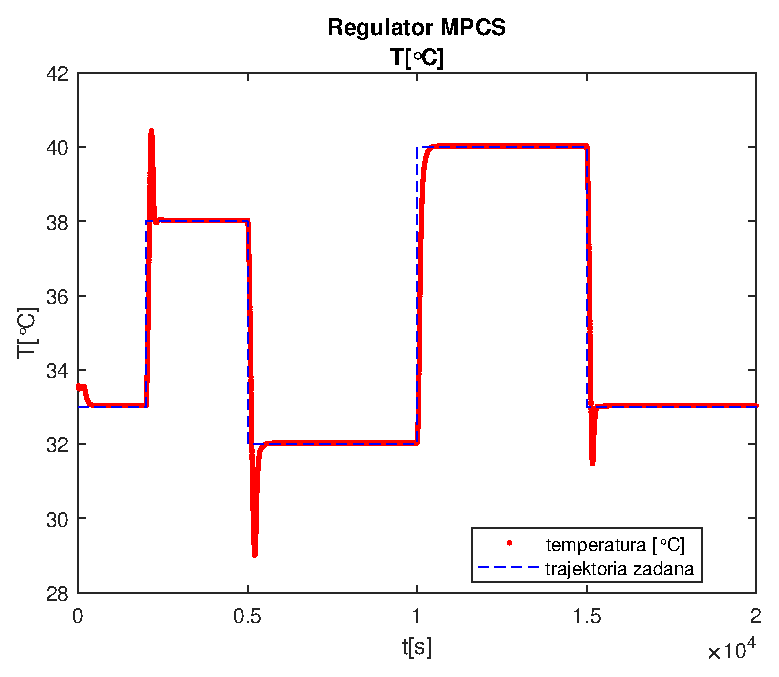
\includegraphics[width=1\linewidth]{img/MPCSanaLin/MPCSLinTN300Nu100l10.eps}
      \caption{}
      \label{fig:fig:MPCSLinN300Nu100l102}
   \end{subfigure}
       
   \begin{subfigure}[b]{0.4\textwidth}
      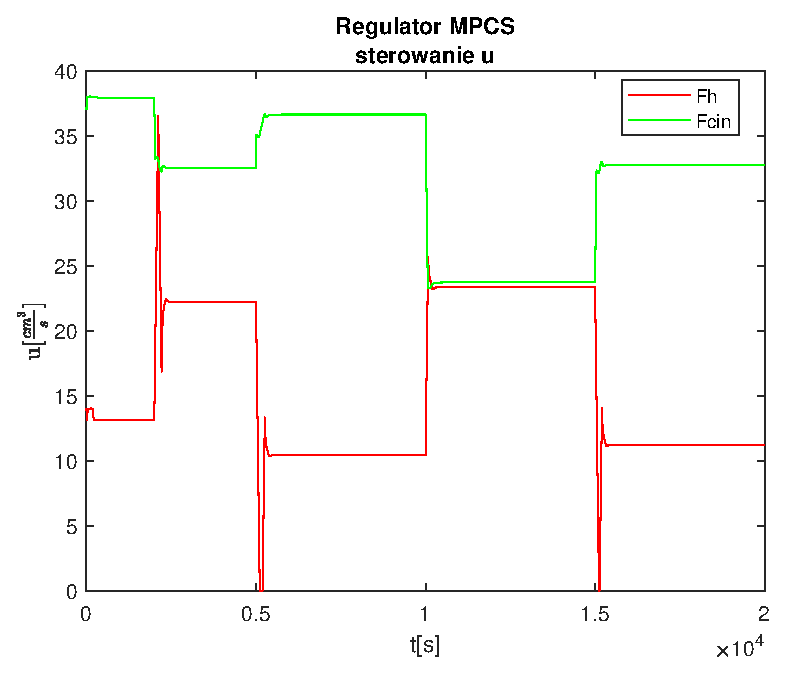
\includegraphics[width=1\linewidth]{img/MPCSanaLin/MPCSLinControlN300Nu100l10.eps}
      \caption{}
      \label{fig:fig:MPCSLinN300Nu100l103}
   \end{subfigure}
       
   \caption{Wykresy dla regulatora MPCS, obiekt liniowy, $N = 300$, $N_u = 100$, $\lambda = 0.1$.}
   \label{fig:MPCSLinN300Nu100l10}
\end{figure}
           

\FloatBarrier

\FloatBarrier
    \begin{figure}[h!]
   \centering
   \begin{subfigure}[b]{0.4\textwidth}
      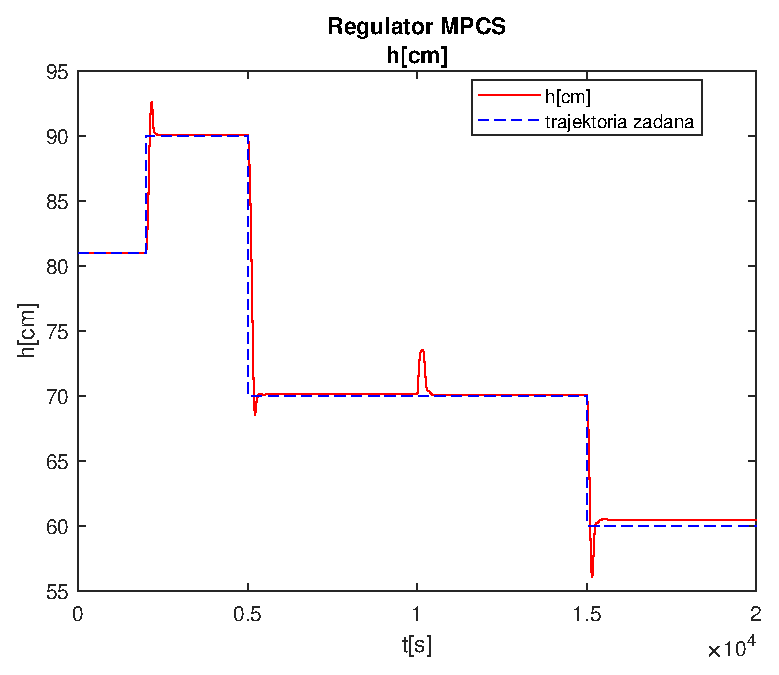
\includegraphics[width=1\linewidth]{img/MPCSanaRK/MPCSRKHN500Nu60l40.eps}
      \caption{}
      \label{fig:fig:MPCSRKN500Nu60l401}
   \end{subfigure}
       
   \begin{subfigure}[b]{0.4\textwidth}
      \includegraphics[width=1\linewidth]{img/MPCSanaRK/MPCSRKTN500Nu60l40.eps}
      \caption{}
      \label{fig:fig:MPCSRKN500Nu60l402}
   \end{subfigure}
       
   \begin{subfigure}[b]{0.4\textwidth}
      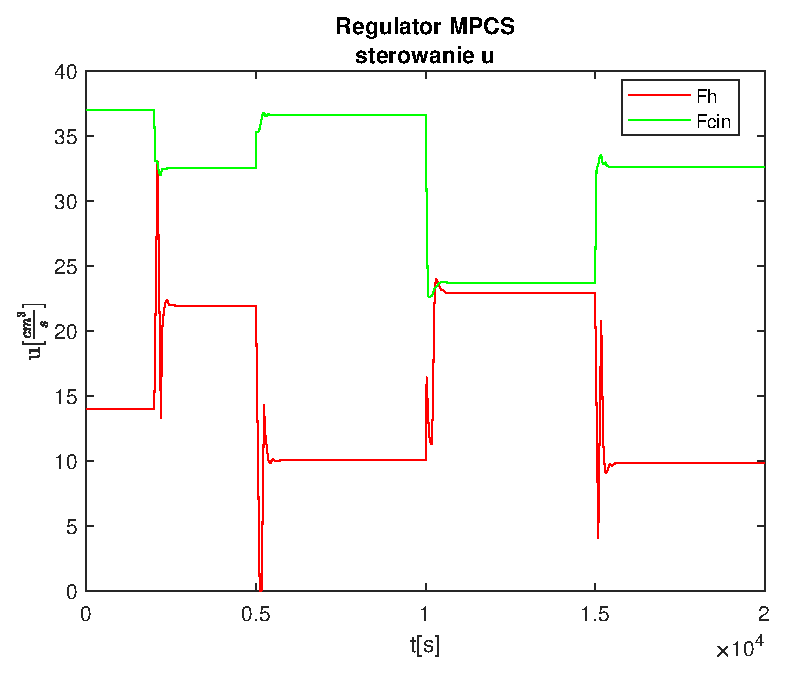
\includegraphics[width=1\linewidth]{img/MPCSanaRK/MPCSRKControlN500Nu60l40.eps}
      \caption{}
      \label{fig:fig:MPCSRKN500Nu60l403}
   \end{subfigure}
       
   \caption{Wykresy dla regulatora MPCS, obiekt nieliniowy.}
   \label{fig:MPCSRKN500Nu60l40}
\end{figure}
           

\FloatBarrier

\FloatBarrier
    \begin{figure}[h!]
   \centering
   \begin{subfigure}[b]{0.4\textwidth}
      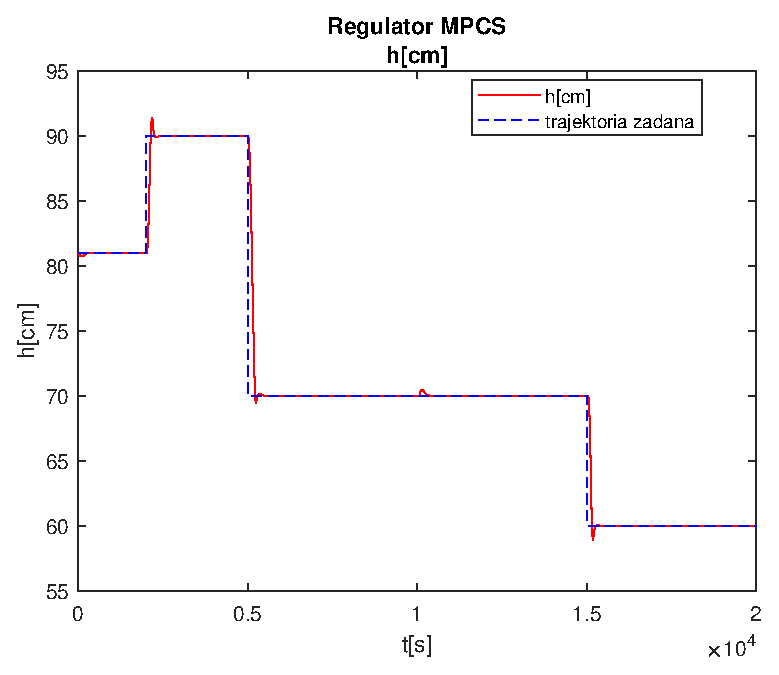
\includegraphics[width=1\linewidth]{img/MPCSanaLin/MPCSLinHN500Nu60l40.eps}
      \caption{}
      \label{fig:fig:MPCSLinN500Nu60l401}
   \end{subfigure}
       
   \begin{subfigure}[b]{0.4\textwidth}
      \includegraphics[width=1\linewidth]{img/MPCSanaLin/MPCSLinTN500Nu60l40.eps}
      \caption{}
      \label{fig:fig:MPCSLinN500Nu60l402}
   \end{subfigure}
       
   \begin{subfigure}[b]{0.4\textwidth}
      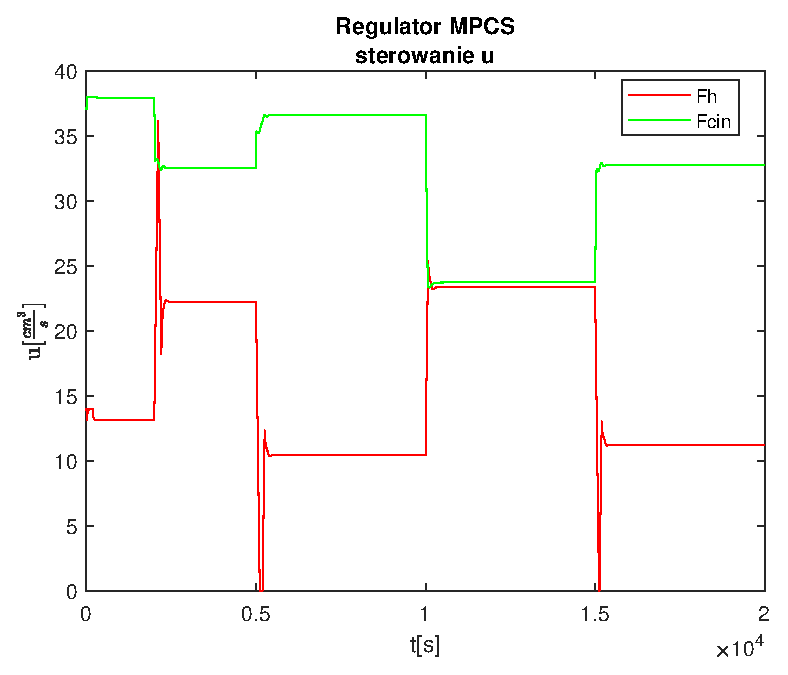
\includegraphics[width=1\linewidth]{img/MPCSanaLin/MPCSLinControlN500Nu60l40.eps}
      \caption{}
      \label{fig:fig:MPCSLinN500Nu60l403}
   \end{subfigure}
       
   \caption{Wykresy dla regulatora MPCS, obiekt liniowy, $N = 500$, $N_u = 60$, $\lambda = 0.4$.}
   \label{fig:MPCSLinN500Nu60l40}
\end{figure}
           

\FloatBarrier